%%%% ijcai23.tex

\typeout{IJCAI--23 Instructions for Authors}

% These are the instructions for authors for IJCAI-23.

\documentclass{article}
\pdfpagewidth=8.5in
\pdfpageheight=11in

% The file ijcai23.sty is a copy from ijcai22.sty
% The file ijcai22.sty is NOT the same as previous years'
\usepackage{ijcai23}

% Use the postscript times font!
\usepackage{times}
\usepackage{soul}
\usepackage{url}
\usepackage[hidelinks]{hyperref}
\usepackage[utf8]{inputenc}
\usepackage[small]{caption}
\usepackage{graphicx}
\usepackage{amsmath}
\usepackage{amsthm}
\usepackage{booktabs}
\usepackage{algorithm}
\usepackage{amsfonts}
% \usepackage{algorithmic}
\usepackage{algpseudocode}
\usepackage[switch]{lineno}
\usepackage{multirow}
\usepackage{subfigure}

% Comment out this line in the camera-ready submission
\linenumbers

\urlstyle{same}

% the following package is optional:
%\usepackage{latexsym}

% See https://www.overleaf.com/learn/latex/theorems_and_proofs
% for a nice explanation of how to define new theorems, but keep
% in mind that the amsthm package is already included in this
% template and that you must *not* alter the styling.
\newtheorem{example}{Example}
\newtheorem{theorem}{Theorem}

% Following comment is from ijcai97-submit.tex:
% The preparation of these files was supported by Schlumberger Palo Alto
% Research, AT\&T Bell Laboratories, and Morgan Kaufmann Publishers.
% Shirley Jowell, of Morgan Kaufmann Publishers, and Peter F.
% Patel-Schneider, of AT\&T Bell Laboratories collaborated on their
% preparation.

% These instructions can be modified and used in other conferences as long
% as credit to the authors and supporting agencies is retained, this notice
% is not changed, and further modification or reuse is not restricted.
% Neither Shirley Jowell nor Peter F. Patel-Schneider can be listed as
% contacts for providing assistance without their prior permission.

% To use for other conferences, change references to files and the
% conference appropriate and use other authors, contacts, publishers, and
% organizations.
% Also change the deadline and address for returning papers and the length and
% page charge instructions.
% Put where the files are available in the appropriate places.


% PDF Info Is REQUIRED.
% Please **do not** include Title and Author information
\pdfinfo{
/TemplateVersion (IJCAI.2023.0)
}

\title{A Relation-specific Entropy-based Ensemble Approach for Knowledge Graph}


% Single author syntax
% \author{
%     Hwawoo Jeon^{1,2}, Yoonseob Lim^{1} and Yong Suk Choi^{2}
%     \affiliations
%     Affiliation
%     \emails
%     email@example.com
% }

% Multiple author syntax (remove the single-author syntax above and the \iffalse ... \fi here)
% \iffalse
\author{
Hwawoo Jeon$^{1,2}$\and
Yoonseob Lim$^{1,3}$\And
Yong Suk Choi$^2$
\affiliations
$^1$Center for Intelligent \& Interactive Robotics\unskip,
Korea Institute of Science and Technology\unskip, 136-791\unskip, Seoul\unskip, Korea\\
$^2$The Division of Computer Science and Engineering\unskip,
Hanyang University\unskip, 04763\unskip, Seoul\unskip, Korea\\
$^3$Department of HY-KIST Bio-convergence\unskip,
Hanyang University\unskip, 04763\unskip, Seoul\unskip, Korea\\
\emails
\{feelgood88, yslim\}@kist.re.kr,
cys@hanyang.ac.kr
}
% \fi

\begin{document}

\maketitle

\begin{abstract}
    Knowledge Graph Embedding(KGE) aims to represent entities and relationships from knowledge graphs(KGs) in vector spaces. Existing KGE methods often focus narrowly on specific patterns, which constrains their inferential capabilities to predict diverse relationship patterns. In response to this limitation, we introduce a relation-specific entropy-based KG ensemble approach, denoted as TransEE. We assume that the entropy of similarity distribution of feature vectors is a reliable indicator of the inference potential for particular relations. On the basis of this hypothesis, TransEE utilizes relation-specific ensemble weights, determined by the entropy of feature vector similarity derived from the base model and independent training data. Moreover, TransEE is designed to be flexible in that it adopts combining base models using normalized entropy measurements in order to effectively be applied to various KG datasets and complex prediction environments. Our experiments on the FB15K and FB15k237 datasets, using four translation-based knowledge graph embedding methods (TransE, TransH, TransR, and TransD) as base models, show that TransEE surpasses both of each single-model and conventional ensemble approaches in terms of prediction accuracy. These results corroborate our hypothesis that the relation-specific entropy of feature vector similarity can take good effect on inference performance of KGE. The code is public at ~\hyperlink{https://github.com/HW-Jeon/TransEE}{https://github.com/HW-Jeon/TransEE}.

\end{abstract}

\section{Introduction}

In artificial intelligence, Knowledge Graphs (KGs) play a pivotal role by structuring and representing extensive knowledge. They represent real-world objects and abstract concepts through entities, relationships, and semantic descriptions. Prominent KGs like FreeBase, WordNet, and DBpedia have been instrumental in various applications, including question-answering and recommendation systems~\cite{10.1093/bib/bbac481,zheng2021knowledge,chen2021topic}.

However, KGs often face the challenge of incompleteness due to the intricate nature of representing the myriad relationships between entities. To address this, knowledge graph embeddings (KGEs) have been proposed. KGEs, employing link-prediction techniques, aim to infer missing links, thereby mitigating KG incompleteness. In this process, KGEs transform KG elements, denoted as triple facts $(h, r, t)$, into a continuous vector space, preserving the KG's structure. The likelihood of a triple is then assessed using a scoring function. Recent advancements have seen the emergence of diverse KGE models, utilizing varied representation spaces and scoring functions: semantic matching models featuring tensor factorization like RESCAL, translational distance models following TransE's translational-principle, complex vector models utilizing complex space as introduced in ComplEx, and models based on neural networks. Despite these developments, no single KGE model has successfully modeling all KG attributes, such as relation patterns (symmetric, anti-symmetric, inverse, composition, hierarchy) and inter-entity (1-to-1, 1-to-N, N-to-1, N-to-N) relationships~\cite{WANG20221041,choi2020approach}. This limitation underscores the need for models that integrate KG information more comprehensively.

Ensemble learning approaches, which generally known to outperform single learners, have seen significant success in machine learning. This concept has been effectively adapted to the context of KGEs, starting with the work of Krompaß and Tresp~\cite{krompass2015ensemble}. Various approaches have been proposed, including committee-based models that derive a final score from a KGEs committee~\cite{choi2020approach}, ensembles of identical KGE models embedded in lower dimensions~\cite{9533372}, and recent methods employing probabilistic ensemble weights~\cite{WANG20221041}.

This paper introduces a novel approach, the ERSE (knowledge graph Ensemble with Relation-Specific Entropy), which focuses on utilizing the entropy of feature vector similarity distributions in each model's vector space rather than individual base-model scores. This methodology stems from the principles of Causal Entropy Force and the proven effectiveness of entropy in complex systems performance evaluation, like the cross-entropy method~\cite{wissner2013causal, de2005tutorial}. In briefly, ERSE extracts triples with specific relations, filtering feature vectors based on each model's prediction ranking, and then calculates relation-specific ensemble weights based on the entropy of these vector distributions. This method, applied to the FB15K and FB15k237 datasets using four translation-based KGE methods(TransE, TransH, TransR, TransD), demonstrates superior predictive accuracy compared to both single-model and general ensemble approaches.

Our paper's contributions include:
\begin{itemize}
    \item We proposing an ensemble mechanism based on the embedded feature vectors in each base model's representation space;
    \item We propose a ensemble approach with entropy as ensemble weights; 
    \item Demonstrating through experiments that the entropy of similarity distribution of feature vectors is a valid indicator of a model's predictive performance.
\end{itemize}


The remainder of this paper is structured as follows: Section 2 reviews related works on KG embedding and ensemble learning. Section 3 details our method. Section 4 presents experimental results and analyses. Concluding remarks are provided in Section 5.



\section{Related Work}

Before proceeding, we introduce our mathematical notations. A triplet is denoted as $(h, r, t)$, with the corresponding column vectors represented by lowercase letters $h$, $r$, $t$. The sets of entities and relations are indicated by uppercase letters $E$ and $R$, respectively. The set $T$, defined as $\{(h, r, t) : h, t \in E, r \in R\}$, comprises these triplets. This set is further divided into three distinct subsets: $T_{train}$, $T_{val}$, and $T_{test}$, corresponding to training, validation, and testing datasets. The score function is expressed as $s(h, r, t)$. Additional notations are elaborated in relevant sections as needed.


\subsection{Translation-based KGE Models}

\textbf{TransE}~\cite{bordes2013translating}. The TransE model initiated the concept of Translation-Based Embedding models. It conceptualizes each relationship as a form of translation within an embedding space. Here, entities and relations are mapped to a low-dimensional vector space, represented as $h$, $r$, $t$. TransE employs the principle $h + r \approx t$ for translating head entities to tail entities, with the score function defined as: $f(h, r, t) = \Vert h + r - t\Vert_2^2$. Although simple and efficient, TransE primarily effective in modeling 1-to-1 relationships, showing limitations in handling 1-to-N, N-to-1, and N-to-N relations.\\
\textbf{TransH}~\cite{wang2014knowledge}. Addressing limitations of TransE, TransH introduces a relation-specific hyperplane, characterized by a normal vector $\textbf{w}_r$ and a translation vector $d_r$. TransH interprets a relation as a translation operation on a specific hyperplane, determined by a normal vector $\textbf{w}_r$ and a translation vector $d_r$. It projects embeddings $h$ and $t$ onto this hyperplane, resulting in $h_\perp = h - \textbf{w}_r^{\top}h\textbf{w}_r$ and $t_{\perp} = t - \textbf{w}_r^{\top}\textbf{w}_r$, followed by the operation $h_\perp + d_r \approx t_\perp$. The score function for TransH is given by $f(h, r, t) = \Vert h + r - t - \textbf{w}_r(\textbf{w}_r^\top(h - t))\Vert_2^2$.\\
\textbf{TransR}~\cite{lin2015learning}. Both TransE and TransH operate under the premise that entity and relation embeddings coexist in the same space. TransR was proposed from the realization that entities and relations, being fundamentally different, might be better represented in separate vector spaces. TransR differentiates entities and relations by assigning a unique mapping matrix $M_r$ for each relation. The score function in TransR is $f(h, r, t) = \Vert M_r h + r - M_r t\Vert_2^2$, where entity embeddings are transformed by the matrix $M_r$ before applying the translational operation. However, TransR can lead to overfitting in simple relations and underfitting in complex relations, due to the uniform parameter learning across different relation complexities.\\
\textbf{TransD}~\cite{ji2015knowledge}. TransD offer solution to address the overfitting of simple relations and underfitting of complex relations observed in TransR. TransD adopts product of two projection vectors instead of projection matrices. It defines the head and tail projection matrices as $M_rh = r_ph_p^\top + I^{d_r \times d_e}$ and $M_rt = r_pt_p^\top + I^{d_r \times d_e}$, respectively, where $d_r$ and $d_e$ represent the dimensions of relation and entity embeddings. Here, $r_p$ is related to relation $r$, and $h_p$, $t_p$ with the related to head and tail entities. This approach reduces parameter load and improves scalability for extensive knowledge graphs.\\
\textbf{TranSparse}~\cite{ji2016knowledge}: The TranSparse model addresses issues of heterogeneity and imbalance in knowledge graphs, which previous translation models have overlooked. Heterogeneity in this context means that various relations link a differing number of entity pairs. Meanwhile, imbalance refers to the unequal numbers of head and tail entities within a relation. To tackle these challenges, TranSparse introduces adaptive sparse matrices instead of standard projection matrices. The sparsity of these matrices is tailored according to the quantity of entity pairs or entities associated with each relation. The score function of TranSparse, $f(h,r,t) = \Vert M^h_r (\theta^h_r)h + r - M^t_r (\theta^t_r)t\Vert_{l1/2}^2$, utilizes these adaptive sparse matrices, where $M^h_r (\theta^h_r)$ and $M^t_r (\theta^t_r)$ represent the matrices for head and tail entities, respectively, with $\theta^h_r$ and $\theta^t_r$ indicating their degrees of sparsity.

As reported by Zhang et al.~\cite{zhang-etal-2022-trans}'s study, translation-based knowledge graph embedding models, classified as translational-distance models by Ji et al.\cite{ji2021survey}, are exhibit a same scoring pattern $\Vert \mathsf{R}_h + r - \mathsf{R}_t \Vert$, where $\mathsf{R}_h$ and $\mathsf{R}_t$ are the deformation of $h$ and $t$ . In this paper, we discuss how to combine multiple models by utilizing traditional translation-based models, i.e., TransE, TransH, TransR, and TransD, which share the same scoring pattern, as base-models instead of other models in improve the performance of KGE.  


% \begin{table}[!tb]
% {
%     \centering
%     \begin{tabular}{ll}
%         \hline
%         Model  & Score Function \\
%         \hline
%         TransE  & $f(h, r, t) = \Vert h + r - t\Vert_2^2$\\
%         TransH  & $f(h, r, t) = \Vert h + r - t - \textbf{w}_r(\textbf{w}_r^\top(h - t))\Vert_2^2$\\
%         TransR  & $f(h, r, t) = \Vert M_r h + r - M_r t\Vert_2^2$\\
%         TransD  & $f(h, r, t) = \Vert M_r (h + r) - M_r (t + r)\Vert_2^2$\\
%         \hline
%     \end{tabular}
%     \caption{Score functions and scoring pattern of translation-based embedding models}
%     \label{tab:score}
% }
% \end{table}

\subsection{Other Models}
\textbf{ComplEx}~\cite{trouillon2016complex}. ComplEx introduces the concept of embedding knowledge graphs (KGs) in a complex space. This is achieved by employing a complex conjugate. Specifically, ComplEx utilizes the real component of a complex bilinear function to denote the likelihood of a positive relationship. The model's scoring function is defined as $f(h, r, t)=Re(\sum_{i=1}^dh_ir_i\bar{t})$, where $\bar{t}$ denotes the complex conjugate of $t$. This scoring mechanism allows for the representation of triples with asymmetric relationships.\\
\textbf{RotatE}~\cite{sun2019rotate}. Introduced to model relationships in four distinct patterns: symmetry, antisymmetry, inverse, and composition, RotatE conceptualizes each relation as a rotational mapping in complex vector space. This is achieved by embedding the source entity $h$ and the target entity $t$ in a complex vector space, based on Euler's formula: $cos\theta + i sin\theta$. The model's effectiveness is evaluated using the score function $f(h,r,t) = \Vert h \circ r - t \Vert$, quantifying the difference between the inner product of $h$ and $r$, and $t$.

\subsection{Ensemble Learning}
Ensemble methods~\cite{zhou2012ensemble} integrate multiple models into a comprehensive model. These methods generally outperform single models and have been successful in various real-world scenarios~\cite{rivas2022ensembles,osamor2021enhancing}. 

These approaches fall into four main categories: voting, bagging, boosting, and combination strategies. Voting and bagging strategies  are similar in that both sample training data for each learner and then integrate the results, but employ distinct methodologies. In voting strategies, diverse algorithms are trained on identical datasets; their predictions are then amalgamated using averaging or majority voting. This approach, known for reducing overfitting risk, requires careful selection of base models and their integration techniques~\cite{a13010026}. A variant, weighted voting, assigns different weights to each model's predictions, demanding strategy for applying reliable weight based on specific objectives~\cite{osamor2021enhancing}.

Bagging, effective for complex models prone to overfitting, trains each model in parallel, substantially reducing variance. This method, exemplified by Random Forest~\cite{breiman2001random}, however, does not decrease bias in underfitting models and demands higher computational resources. Boosting methods, such as  Adaboost~\cite{freund1996experiments}, iteratively adjust the training data distribution based on previous outputs, enhancing learner performance. Combinatorial strategies independently train learners and merge outcomes through averaging, voting, or additional learners.

Krompaß and Tresp~\cite{krompass2015ensemble} first explored this concept in KGE models, establishing that ensemble predictions outperformed those from individual base models. More recently, Xu et al.~\cite{9533372} demonstrated enhanced performance in KGE models through parallel training at lower dimensions and aggregating scores, compared to training a single higher-dimension model. Additionally, Wang et al.~\cite{WANG20221041} proposed combining different embedding model scores using probabilistic weights, providing a theoretical framework for optimal parameter calculation in ensemble models and predicting link prediction rates.More resently, Wang et al.~\cite{WANG20221041} presented to combine the scores of different embedding models by using a probabilistic weights and theoretical framework to calculate the optimal parameters for the ensemble model and predict its corresponding link prediction rate.

\section{Method}

\bgroup
\begin{figure*}[t]
  \centering \makeatletter\IfFileExists{Images/Figure1_v2.png}{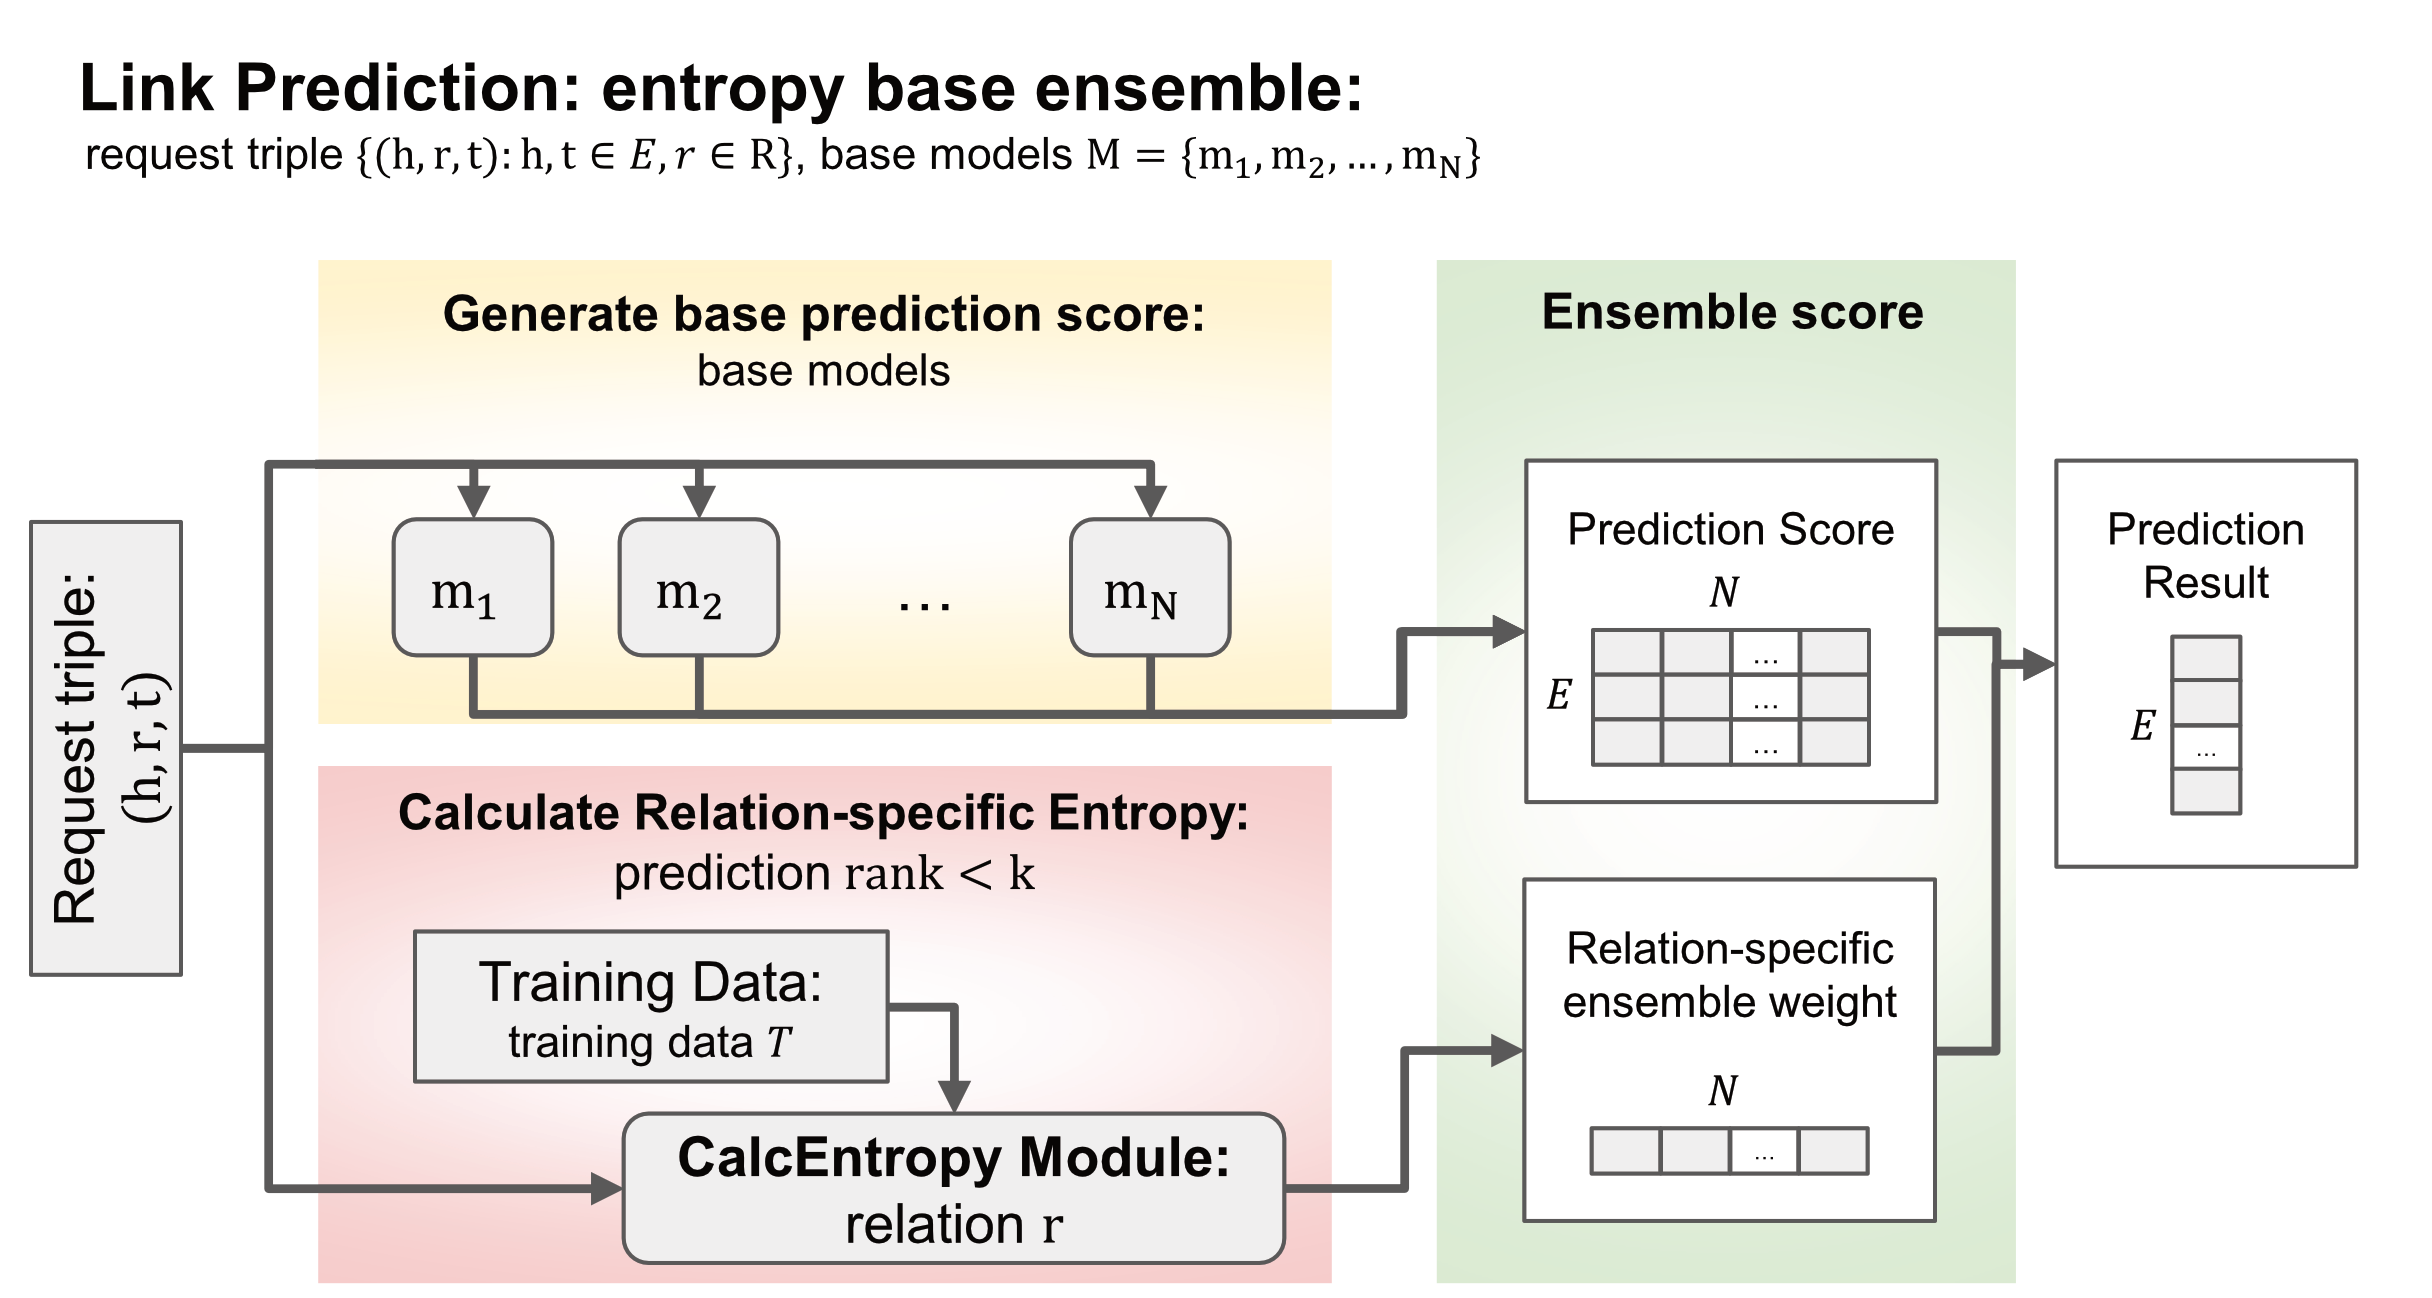
\includegraphics[width =0.75\textwidth]{Images/Figure1_v2.png}}{}
  \makeatother
  \caption{{Overview of link-prediction sequence: entropy base ensemble}}
  \label{fig:sysArch}
  \hfill
\end{figure*}
\egroup

In the this section, we detail the ERSE (knowledge graph Ensemble with Relation-Specific Entropy) approach, designed for enhancing link prediction in knowledge graphs. This approach is predicated on the hypothesis that the entropy of similarity distributions in feature vectors is a reliable indicator of a model's predictive performance. This method utilizes relation-specific entropy weights to ensemble multiple translation-based Knowledge Graph Embeddings (KGEs). The process begins with the computation of base prediction scores for each model in the ensemble, followed by the calculation of relation-specific entropy. The entropy is derived from the distribution of feature vectors' similarity, which is based on the models' prediction ranking and training dataset. The calculated entropy then guides the determination of ensemble weights for each model. The final prediction score is a sum of the weighted scores from all models. This methodology is distinct in its focus on the entropy of feature vector similarity distributions within each model's vector space. The algorithmic steps, including inputs, outputs, and procedures, are elaborately illustrated in Figure ~\ref{fig:sysArch} and Algorithm ~\ref{alg:linkPredictOverview}. 

\begin{algorithm}[!htb]
    \caption{Link Prediction: entropy base ensemble}
    \label{alg:linkPredictOverview}
    \textbf{Input}: Request triple $\{(h, r, t) \;:\; h,t \in E, r \in R\}$, base models $\{\mathcal{M}_i \;:\; i \in N\}$, minimum number of vectors $minLen$ for weight reliability, type of entropy normalization $norm$, type of entropy $\mathit{type}$, type of distance $\mathit{dist}$, hit rank threshold $k$, and min-max range of normalization for prediction score $\delta^{s}$ and ensemble weight $\delta^{w}$.\\
    \textbf{Output}: Ensemble prediction Score $\mathcal{S}$.
    
    \begin{algorithmic}[1] %[1] enables line numbers    

        \Statex \hrulefill
        \Statex \textbf{Link-prediction sequence}
        \Statex \noindent$\overline{\makebox[\linewidth]{\text{Generates Base Prediction Score:} $s\acute{}$ \hfill}}$
        
        \State $s\acute{}_i \leftarrow \{\mathcal{N}_{\text{minmax}}(f^i(h, r, t), \delta^{S}) \;|\; \forall i \in N\}$    
        \Statex Calculate Relation-specific Entropy $\mathcal{H}$ and their number of resource vector: $resSize$.
        \State $\mathcal{H}, resSize \leftarrow \Call{CalcEntropy}{\mathcal{M}, r}$

        \Statex Ensemble for Final Prediction Score: $\mathcal{S}$.
        \State $\mathcal{W}^i \leftarrow \{\mathcal{N}_{norm}(\mathcal{H}^i, \delta^{W}) \;|\; resSize^{i}>minLen\}$

        \If{$\Call{Len}{\mathcal{W}} < 1$}
            \State $\mathcal{W}^i \leftarrow \{1\;|\; \forall i \in N\}$
        \EndIf
        
        \State $\mathcal{S} \leftarrow \sum_{m=1}^{N} s\acute{}_i \mathcal{W}i$
        \State \Return $\mathcal{S}$
        
        \Statex \hrulefill
        \Statex \noindent\underline{\hbox to \linewidth{\textbf{Relation-specific entropy calculation}\hfill}}

        \Function{CalcEntropy}{$\mathcal{M}, \hat{r}, k, type, dist, norm, \delta^w$}

            \State $\hat{T} \leftarrow \{(h,\hat{r},t)\;|\; \forall (h,\hat{r},t) \in T_{train}\}$
            \State $res^{i} \leftarrow \{\mathcal{V}^i(h,\hat{r},t) \;|\;\mathrm{avg}(\mathrm{rank}(h,\hat{r},t)) <k,$
            \Statex \hspace{3.5em}$(h,\hat{r},t) \in \hat{T}, \forall i \in N\}$
        
            \For{$i$ in $N$}
                \State ${res^{i}} \leftarrow \mathrm{drop}(res^{i}, \mathrm{min}(\mathrm{len}(res)))$
                \State $prob^{i} \leftarrow Probs(D_{\mathit{dist}}(res^{i}, res^{i}))$
                \State $\mathcal{E}^{i} \leftarrow \mathcal{H}^{\mathit{type}}(prob_r^m)$
                \State $resSize^{i} \leftarrow \mathrm{len}(res^{i})$  
            \EndFor
            \State \Return $\mathcal{E}, resSize$
        \EndFunction
    \end{algorithmic}
\end{algorithm}

\subsubsection{Request for Link-Prediction}

The ERSE takes as input a request triple $\{(h, r, t) : h, t \in E, r \in R\}$, where $E$ represents the set of entities including head and tail entities $h$ and $t$, and $R$ denotes the set of relations containing $r$. The algorithm also utilizes base models $\{\mathcal{M}_i : i \in N\}$, where $i$ is the index of base model and $N$ is the number of base models, along with a series of hyperparameters: 
\begin{itemize}
    \item $minLen$: Minimum number threshold of resource vectors to ensure reliability of relationship-specific entropy as a performance indicator;
    \item $k$: Maximum rank threshold of resource vectors to ensure reliability of relationship-specific entropy as a performance indicator;
    \item $dist$: Type of pairwise distance metric to computation for similarity distribution of feature vectors;
    \item $type$: Indicator of type of entropy formula to apply for relation-specific entropy computation;
    \item $norm$: Indicator of type of normalization method to apply for relation-specific entropy;
    \item $\delta^s$: Min-max range of normalized prediction score;
    \item $\delta^w$: Min-max range of normalized ensemble weight. 
\end{itemize}
Additionally, Two types of normalization methods are used to normalization of base prediction score and relation-specific entropy:
\begin{align}
\label{eq:NormMM}
    \mathcal{N}_{\text{minmax}}(X, \delta) = \delta_{min} + \delta_{scale}*\frac{x_{ij} - \min(X)}{\max(X) - \min(X)},
\end{align}%

\begin{align}
\label{eq:NormLogit}
    \mathcal{N}_{\text{logit}}(X, \delta) =  \delta_{min} + \delta_{scale}*\log\left(\frac{x}{1 - x}\right),
\end{align}%
where $X$ represents the set of data, with $\delta_{min}$ and $\delta_{scale}$ being the minimum value and scale value, respectively.

\subsubsection{Generates Base Prediction Score}
In the initial step of link prediction, each base model, denoted as $\mathcal{M}_i$, computes a prediction score $s\acute{}_i$ for the input triple using its respective score function $f(h,r,t)$. These scores undergo normalization by the min-max method $\mathcal{N}_{\text{minmax}}(X, \delta^s)$, as outlined in Equation \ref{eq:NormMM}. The normalization process ensures that the scores from different models are scaled uniformly, facilitating a fair combination in the subsequent steps.

\subsubsection{Calculate Relation-Specific Entropy}
To determine the ensemble weight specific to a relation, we calculate its relation-specific entropy, a vital component of the algorithm, denoted as $\Call{CalcEntropy}$ in Algorithm \ref{alg:linkPredictOverview}. This function takes as input a set of base models $\mathcal{M}$, a target relation $\hat{r}$, and various hyperparameters: $k, type, dist, norm, \delta^w$. \\
\textbf{Filtering Training Triple}: The process of computing relation-specific entropy begins with the step of filtering out triples that contain the target relation, denoted as $\hat{r}$, from the training dataset $T_{train}$, thereby generating $\hat{T}$. \\
\textbf{Relation-specific Feature Vectors}: Subsequently, It calculates the link prediction rank $rank(h, \hat{r}, t)$ for each triplet in the training data involving local target relation $\hat{r}$ by $i$-th model. The predicted feature vectors $\{res^i \;:\; i \in N\}$, filtered by the average rank and a predefined hit rank threshold $k$, allow for utilize the evaluate of each model’s predictive accuracy for $\hat{r}$. Specifically, In this sequence, the difference in length of each $res^i$ impacts the entropy. Because TransEE computes the relation-specific entropy based on these $res^i$, this difference negative affecting the performance and reliability of the ensemble weights. As detailed in line 13 of the Algorithm ~\ref{alg:algorithm}, to ensure the reliability of ensemble weights for indicating each model's predictive performance for a relation, TransEE harmonizes other $res^i$ to match the smallest length among the $res^i$, as executed by the $\mathrm{drop}$ function. The extraction method varies across models, exemplified by the TransE model~\cite{bordes2013translating}, defined as:
\begin{align}
\label{eq:PreV}
    \mathcal{V}^{TransE}(h, r, t) = \begin{cases}
            t-r & \text{, when head prediction} \\
            h+r & \text{, when tail prediction} \\
        \end{cases}.
\end{align}%
\textbf{Pairwise distances}: Pairwise distances $D_{\mathit{dist}}(res^{i}, res^{i})$ are then computed, utilizing methods such as Euclidean or cosine distance. In this study, we employ both Euclidean and cosine distance, defined as:
\begin{align}
\label{eq:DistEu}
    \mathcal{D}_{\text{euclidean}}(A_i, A_j) = \sqrt{\sum_{k=1}^{m}(A_{ik} - A_{jk})^2},
\end{align}%
\begin{align}
\label{eq:DistLogit}
    \mathcal{D}_{\text{cosine}}(A_i, A_j) = 1 - \frac{\sum_{k=1}^{m}A_{ik} \times A_{jk}}{\sqrt{\sum_{k=1}^{m}A_{ik}^2} \times \sqrt{\sum_{k=1}^{m}A_{jk}^2}}.
\end{align}%
\textbf{Distribution Similarity of Feature Vector}:
To incorporate feature vector similarity into entropy calculations, the algorithm uses a model-specific probability distribution  $prob^i$  to analyze distance probabilities. We adopt the Burr distribution~\cite{burr1942cumulative}, formulated as:  
\begin{align}
\label{eq:PDF}
    Probs(x; c, d) = cd \frac{x^{c-1}}{(1 + x^c)^{d+1}},        
\end{align}%
where $x \geq 0$ is a variable, $c > 0$ and $k > 0$ are shape parameters. In Figure ~\ref{fig:pdfhist}, we present a example of pairwise distances and probability density function for the Burr distribution. This figure compares the Euclidean and cosine similarities within the TransD model, focusing on a specific relation from the FB15k237 dataset. 
\bgroup
\begin{figure}[b!]
  \centering \makeatletter\IfFileExists{Images/Figure2.png}{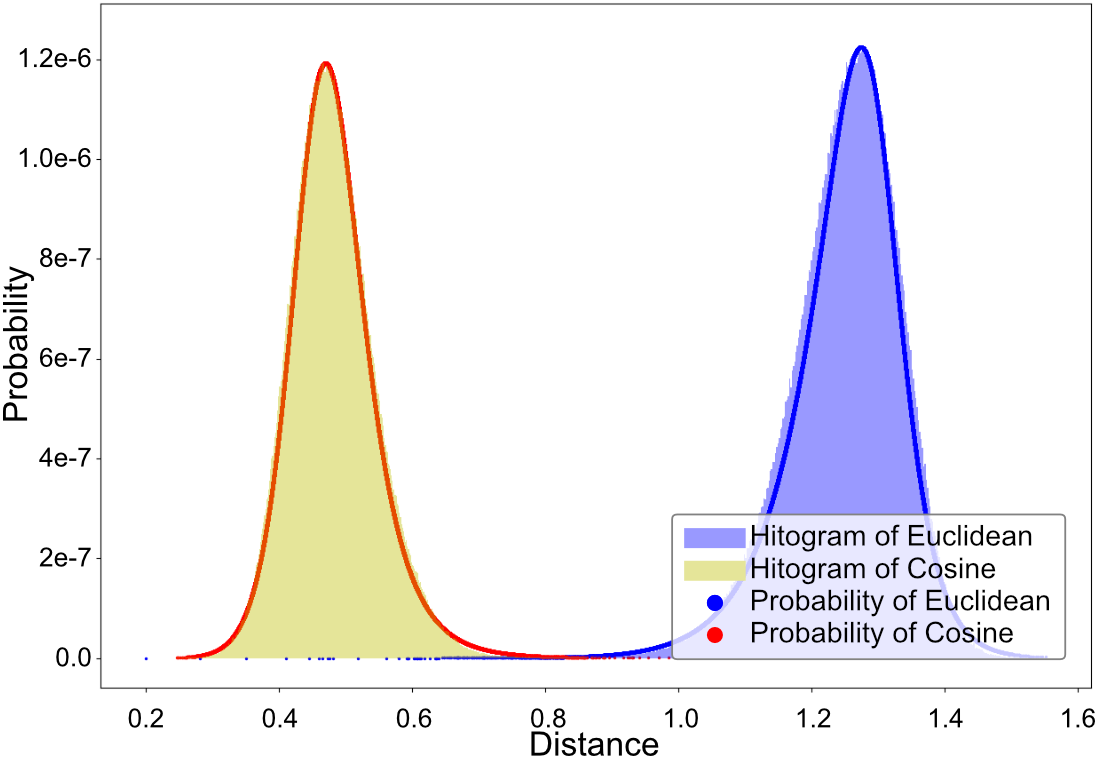
\includegraphics[width =0.48\textwidth]{Images/Figure2.png}}{}
  \makeatother
  \caption{{Compare of probability density function and pairwise distance histogram; TransD and relation $14$.}}
  \label{fig:pdfhist}
  \hfill
\end{figure}
\egroup
\textbf{Relation-specific Entropy}: The algorithm then calculates the relation-specific entropy ${\mathcal{H}^{i} \;:\; i \in N}$ based on the selected $type$ of entropy. Adopted of entropy types include Shannon and Rényi, defines as:
\begin{align}
    \label{eq:shannon}
    \mathcal{H}^{shannon}(X) = -\sum_{i} p(x_i) \log p(x_i), 
\end{align}%
\begin{align}
    \label{eq:Rényi}    
    \mathcal{H}_{\alpha}^{r\acute{e}nyi}(X) = \frac{1}{1-\alpha} \log \left( \sum_{i} p(x_i)^\alpha \right).
\end{align}%
The function, which driven by parameter $type$ as a type of entropy, return the entropy result $\mathcal{H}$ and the resource size count $\{resSize^{i} \;:\; i \in N\}$ and provide a quantitative basis for determining relation-specific ensemble weight. 

Notably, relation-specific entropy calculation method operates independently from the actual link prediction process and accommodates pre-trained models, enhancing flexibility in base model combinations. This allows for either a one-time computation during link prediction or pre-computation for each relation, optimizing computational resources and expediting the link prediction process.

\subsubsection{Ensemble for Final Prediction Score}
Final step, based on relation-specific entropy and base score, TransEE determines ensemble weight and compute prediction score. Relation-specific ensemble weights $mathcal{W}^i$ are determined for each model in the ensemble. These weights are derived by normalizing the relation-specific entropy $\mathcal{H}^i$ using Equation~\ref{eq:NormMM,eq:NormLogit} with the normalization parameter(i.e. $norm$ and $\delta^{W}$), but only for those models where the number of resource vectors \(resSize^{i}\) exceeds the defined minimum length \(minLen\). If the ensemble ends up without any weights (\(\Call{Len}{\mathcal{W}} < 1\)), a default weight of 1 is assigned to each model in the ensemble (\(\mathcal{W}^i \leftarrow \{1\;|\; \forall i \in N\}\)). This step ensures that each model contributes equally to the final prediction in the absence of significant relation-specific entropy. Finally, the ensemble prediction score \(\mathcal{S}\) is computed as the sum of the products of each model's base prediction score \(s\acute{}_i\) and its corresponding weight \(\mathcal{W}i\). The computed score \(\mathcal{S}\) is then returned as the output of the algorithm.


% 절차는 
% 1. 각 모델의 Score를 구한다. 이때, 각 모델의 Score는 각각 normalize 된다.
% 2. 요청된 relation에 따라 각 모델의 entropy 값을 구하고 이를 normalize 한다.
% 2-1. 우리는 이를 위해 MIN-MAX Normlaize와 Logit Normalize 두가지 방식을 사용하여 그 성능을 비교하였으며, 각 수식은:







\section{Experiments and Results Analysis}
\subsection{Datasets}

In evaluate the performance of our approach, we utilized two benchmark Knowledge Graphs (KGs) derived from Freebase~\cite{10.1145/1376616.1376746}: FB15K~\cite{NIPS2013_1cecc7a7} and FB15K237~\cite{toutanova-chen-2015-observed}. FB15K consists of a subset of knowledge triples from the extensive Freebase database, covering a range of topics including sports, actors, movies, and more. Most test triples in FB15K can be inferred by their inverse triples in the training dataset. In contrast, FB15K237, a modified version of FB15K, excludes inverse relations, presenting a more challenging scenario for link prediction as it demands more advanced modeling. Table ~\ref{tab:datasets} provides a comprehensive overview of these datasets.

\begin{table}[hbtp!]
{
    % \small
    \centering
    \begin{tabular}{cccccc}
        \toprule
        \textbf{Dataset} & \textbf{\#Ent} & \textbf{\#Rel} & \textbf{\#Train}  & \textbf{\#Valid.} & \textbf{\#Test}\\
        \midrule

        FB15K & 14951 & 1345 & 483142 & 50000 & 59071\\
        FB15K237 & 14541 & 237 & 272115 & 17535 & 20466\\
        
        \bottomrule
    \end{tabular}
    \caption{Score functions of translation-based embedding models}
    \label{tab:datasets}
}
\end{table}

\subsection{Experiment Settings}

\subsubsection{Implementation details}
To evaluate the efficacy of TransEE, four metrics are utilized: Hits@K (with K values of 1, 3, and 10) to gauge accuracy in top K predictions, and Mean Reciprocal Ranking (MRR), where higher Hits@K and MR signify enhanced performance. TransEE is implemented using Pytorch 2.0.0, on an Ubuntu 20.04 operating system, with a single NVIDIA RTX4090 GPU and an AMD Ryzen 9 5950x processor, backed by 64GB of RAM.

The study report the results of eight TransEE variants, distinguished by their combination of methods: entropy normalization (min-max or logit~\cite{berkson1944application}), entropy calculation (Shannon~\cite{shannon1948mathematical} or Rényi~\cite{renyi1961measures}), and pairwise distance measurement (Euclidean or cosine).

In adherence to the widely-recognized filtered setting approach~\cite{bordes2013translating}, corrupted triplets in train, valid, and test sets were excluded. We also implemented and utilized an ensemble method, combining four typical translation-based knowledge graph embedding models, i.e. TransE, TransH, TansR and TransD, using the OpenKE~\cite{han-etal-2018-openke} framework for base model training before ensemble integration. The base models shared the same embedding dimension, with other hyperparameters set to OpenKE defaults. The implementation code and hyperparameters are available at ~\hyperlink{https://github.com/HW-Jeon/TransEE}{https://github.com/HW-Jeon/TransEE}, along with used hyperparameters.

\subsubsection{Baseline}
TransEE's efficacy is compared against two baselines to demonstrate our ensemble method's performance. The baselines include: (1) KGE methods: TransE~\cite{bordes2013translating}, TransH~\cite{wang2014knowledge}, TransR~\cite{lin2015learning}, TransD~\cite{ji2015knowledge};  (2) A general ensemble method, denoted as $ScoreSum$, which aggregates the scores of each model, $\mathcal{S} \leftarrow \sum_{m=1}^{N} s\acute{}_i$.


% \subsection{Link Prediction}
% [† ]: results are taken from corresponding original paper

\subsubsection{Experimental Results of Link Prediction}
The goal of link prediction is to identify the missing head or tail entity (h or t) in a triplet (h, r, t). For this, we eliminate either the head or tail entity from each triplet in the test set and substitute it with every entity in the dictionary, sequentially. These modified triplets are then scored, and ranked in descending order based on their scores. The focus here is on the rank of the correct entity rather than simply identifying the top entity.

The link prediction performance of TransEE in comparison to baseline models is presented in Table ~ref{tb:ExpResult}. TransEE exhibits enhanced performance across MRR, Hits@1, Hits@3, Hits@10 metrics, surpassing all baseline models. In particular, TransEE showed an improvement over the common ensemble method, $ScoreSum$, even though the $ScoreSum$ method was observed to consistently outperform the base model depending on the prediction ability of each model. Specifically, on the datasets FB15K and FB15K237, TransEE shows improvements of 2.98\% and 0.79\% in MRR, and 3.25\% and 0.75\% in Hits@1, respectively, compared to the general ensemble method $ScoreSum$. These results affirm the utility of relation-specific entropy as an effective ensemble weight in TransEE's methodology.

\begin{center}
\begin{table*}[tb!]
{
    \centering 
    \begin{tabular}{c|c|cccc|cccc}
        \toprule
        \multicolumn{1}{c|}{} & \multicolumn{1}{c|}{\textbf{Dataset}} & \multicolumn{4}{c|}{\textbf{FB15K}} & \multicolumn{4}{c}{\textbf{FB15K237}} \\ 
        \midrule
        & \textbf{Model} & {MRR} & {Hits@1} & {Hits@3} & {Hits@10} & {MRR} & {Hit@1} & {Hit@3} & {Hit@10}\\
        \midrule
        & TransE & 0.3907 & 0.2700 & 0.4539 & 0.6126 & 0.2882 & 0.1905 & 0.3277 & 0.4859 \\ %& 0.2050 & 0.0129 & 0.3681 & 0.4773 \\
        & TransH & 0.4591 & 0.3287 & 0.5400 & 0.6890 & 0.289 & 0.1874 & 0.3316 & 0.4877  \\ %& 0.2028 & 0.0116 & 0.3701 & 0.4734 \\
        & TransR & 0.4649 & 0.3326 & 0.5487 & 0.6969 & 0.2911 & 0.1954 & 0.3292 & 0.4829 \\ %& 0.2138 & 0.0166 & 0.3894 & 0.4679 \\
        & TransD & 0.5139 & 0.3767 & 0.6098 & 0.7391 & 0.2915 & 0.1922 & 0.3311 & 0.4891 \\ %& 0.2040 & 0.0247 & 0.3551 & 0.4738 \\
        \midrule
        & \footnotesize	$ScoreSum$ & 0.5158 & 0.3882 & 0.6005 & 0.7307 & 0.3177 & 0.2136 & 0.3629 & 0.5218 \\ %& 0.2154 & 0.0158 & 0.3909 & 0.4860 \\
        \midrule
        \multirow{4}{*}{\rotatebox[origin=c]{90}{TransEE}}
        % \hspace{0.01em}
        \multirow{4}{*}{\rotatebox[origin=c]{90}{\scriptsize($Shannon$)}}
        & \footnotesize $Euclidean+MinMax$ & 0.5337 & \underline{0.4056} & 0.6217 & 0.7467 & \textbf{0.3203} &  \textbf{0.2158} &  0.3658 &  0.5254 \\ %&&&& \\        
        & \footnotesize $Euclidean+Logit$ & 0.5336 & 0.4053 & 0.6217 & 0.7463 & \underline{0.3203} &  0.2157 &  \textbf{0.3661} &  0.5250\\ %&&&& \\
        & \footnotesize $Cosine+MinMax$ & 0.5336 & 0.4054 & 0.6217 & \textbf{0.7467} & 0.3194 &  \underline{0.2145} & 0.365 &  0.5250\\
        & \footnotesize $Cosine+Logit$ & 0.5335 & 0.4051 & 0.6217 & 0.7463 & 0.3195 &  0.2145 &  0.3654 &  0.5254\\
        
        \midrule
        % \cmidrule(rl){1-1}
        
        \multirow{4}{*}{\rotatebox[origin=c]{90}{TransEE}}
        \multirow{4}{*}{\rotatebox[origin=c]{90}{\scriptsize($Re\acute{}nyi$)}}
        & \footnotesize $Euclidean+MinMax$ & \textbf{0.5337} & \textbf{0.4056} & 0.6217 & 0.7467 & 0.3203 &  0.2157 &  0.3655 &  0.5255 \\
        & \footnotesize $Euclidean+Logit$  & \underline{0.5337} & 0.4054 & 0.6217 & 0.7462 & 0.3202 & 0.2155 & \underline{0.3659} & 0.5254\\
        & \footnotesize $Cosine+MinMax$ & 0.5337 & 0.4055 & \underline{0.6217} & \underline{0.7467} & 0.3196 &  0.2146 &  0.3654 &  \underline{0.5255} \\ 
        & \footnotesize $Cosine+Logit$ & 0.5336 & 0.4052 & \textbf{0.6218} & 0.7463 & 0.3195 & 0.2143 & 0.3654 & \textbf{0.5258}\\

        
        \midrule
        & Relative $\uparrow$ & \textbf{3.47}\% & \textbf{4.49}\% & \textbf{3.53}\% & \textbf{2.19}\% & \textbf{0.81}\% & \textbf{1.01}\% & \textbf{0.78\%} & \textbf{0.67}\% \\
        
        \bottomrule
    \end{tabular}
    \caption{Results of link prediction on datasets FB15K and FB15K237. The \textbf{best} and \underline{second-best} scores in each column are emphasized. The row of Relative $\uparrow$ indicates the comparative link prediction performance between $ScoreSum$ and the optimal variant of TransEE for each dataset.}
    \label{tb:ExpResult}
}
\end{table*}
\end{center}

% & 0.5337 & 0.4056 & 0.6217 & 0.7467
% & 0.5336 & 0.4053 & 0.6217 & 0.7463
% & 0.5336 & 0.4054 & 0.6217 & 0.7467
% & 0.5335 & 0.4051 & 0.6217 & 0.7463
% & 0.5337 & 0.4056 & 0.6217 & 0.7467
% & 0.5337 & 0.4054 & 0.6217 & 0.7462
% & 0.5337 & 0.4055 & 0.6217 & 0.7467
% & 0.5336 & 0.4052 & 0.6218 & 0.7463


% 0.5337 & 0.4056 & 0.6217 & 0.7467

% FB15K - mm/eu/shannon
% 0.5337 & 0.4056 & 0.6217  & 0.7467			
% 3.47033734	4.482225657	3.530391341	2.189681128

% // minmax-c_renyi - in FINAL N FB15K237
% 0.3194 & 0.2143 & 0.3653 & 0.5257 	
Further, when analyzing the Hits@10 for different relation types, Table ~\ref{tb:REResult} details these results, categorizing them by the properties of relations in FB15k and FB15K237 datasets. These findings highlight TransEE's superior performance over the baselines. In FB15K and FB15K237, improvements are evident in Hits@10 (3.25\% and 0.75\%) relative to $ScoreSum$. This underscores the efficacy of relation-specific entropy in enhancing TransEE's ensemble weighting methodology.

\begin{center}
\begin{table*}[htb!]
{
    \centering
    \begin{tabular}{c|c|cccc|cccc}
        \toprule
        \multicolumn{1}{c}{} & \multicolumn{1}{c|}{\textbf{Dataset}} & \multicolumn{4}{c|}{\textbf{FB15K(Hits@10)}} & \multicolumn{4}{c}{\textbf{FB15K237(Hits@10)}} \\ 
        \midrule
        & \textbf{Model} & \textbf{1-to-1} & \textbf{1-to-N} & \textbf{N-to-1} & \textbf{N-to-N} & \textbf{1-to-1} & \textbf{1-to-N} & \textbf{N-to-1} & \textbf{N-to-N} \\
        \midrule
        & TransE & 0.8191 & 0.6389 & 0.6118 & 0.6057 & 0.5599 & 0.3623 & 0.4951 & 0.4858 \\ %& 0.2050 & 0.0129 & 0.3681 & 0.4773 \\
        & TransH & 0.8564 & 0.6813 & 0.6424 & 0.6959 & 0.5599 & 0.3461 & 0.4900 & 0.4985  \\ %& 0.2028 & 0.0116 & 0.3701 & 0.4734 \\
        & TransR & 0.9177 & 0.7173 & 0.6845 & 0.7476 & 0.5990 & 0.3256 & 0.4959 & 0.4915 \\ %& 0.2138 & 0.0166 & 0.3894 & 0.4679 \\
        & TransD & 0.8684 & 0.6919 & 0.6546 & 0.7011 & 0.5521 & 0.3531 & 0.4910 & 0.4997 \\ %& 0.2040 & 0.0247 & 0.3551 & 0.4738 \\
        \midrule
        & \footnotesize	$ScoreSum$ & 0.9032 & 0.7185 & 0.6760 & 0.7396 & 0.5833 & 0.3797 & 0.5207 & 0.5338 \\ %& 0.2154 & 0.0158 & 0.3909 & 0.4860 \\
        \midrule
        \multirow{4}{*}{\rotatebox[origin=c]{90}{TransEE}}
        % \hspace{0.01em}
        \multirow{4}{*}{\rotatebox[origin=c]{90}{\scriptsize($Shannon$)}}
        & \footnotesize $Euclidean+MinMax$ & \textbf{0.9249} & 0.7279 & 0.6848 & 0.7577 & \textbf{0.5885} & 0.3778 & 0.5215 & 0.5385 \\ 
        & \footnotesize $Euclidean+Logit$ & 0.9237 & 0.7278 & 0.6848 & 0.7571 & \textbf{0.5885} & 0.3801 & 0.5211 & 0.5379 \\ 
        & \footnotesize $Cosine+MinMax$ & \underline{0.9243} & \underline{0.7279} & 0.6843 & \textbf{0.7578} & \underline{0.5859} & 0.3809 & 0.5210 & 0.5379 \\ 
        & \footnotesize $Cosine+Logit$ & 0.9237 & 0.7278 & \underline{0.6849} & 0.7571 & \underline{0.5859} & \textbf{0.3821} & 0.5209 & 0.5385 \\ 
        
        \midrule
        % \cmidrule(rl){1-1}
        
        \multirow{4}{*}{\rotatebox[origin=c]{90}{TransEE}}
        \multirow{4}{*}{\rotatebox[origin=c]{90}{\scriptsize($Re\acute{}nyi$)}}
        & \footnotesize $Euclidean+MinMax$ & \underline{0.9243} & 0.7278 & 0.6847 & 0.7577 & \underline{0.5859} & 0.3778 & 0.5211 & \textbf{0.5388} \\ 
        & \footnotesize $Euclidean+Logit$  & 0.9237 & 0.7278 & 0.6848 & 0.7571 & \textbf{0.5885} & 0.3766 & \underline{0.5219} & 0.5385 \\ 
        & \footnotesize $Cosine+MinMax$ & \underline{0.9243} & \textbf{0.7281} & 0.6845 & \underline{0.7577} & \underline{0.5859} & \underline{0.3817} & 0.5211 & 0.5385 \\ 
        & \footnotesize $Cosine+Logit$ & 0.9237 & 0.7278 & \textbf{0.6850} & 0.7572 & \underline{0.5859} & 0.3790 & \textbf{0.5227} & \underline{0.5387} \\ 
        
        \bottomrule
    \end{tabular}
    \caption{Results of link prediction on datasets FB15K and FB15K237. The \textbf{best} and \underline{second-best} scores in each column are emphasized. The row of Relative $\uparrow$ indicates the comparative link prediction performance between $ScoreSum$ and the optimal variant of TransEE for each dataset.}
    \label{tb:REResult}
}
\end{table*}
\end{center}

% 0.8191 & 0.6389 & 0.6118 & 0.6057
% 0.8564 & 0.6813 & 0.6424 & 0.6959
% 0.9177 & 0.7173 & 0.6845 & 0.7476
% 0.8684 & 0.6919 & 0.6546 & 0.7011


\section{Conclusion and Future Work}

\section*{Acknowledgments}

%% The file named.bst is a bibliography style file for BibTeX 0.99c
\bibliographystyle{named}
\bibliography{ijcai23}

\end{document}
